
\documentclass[envcountsect]{beamer}
\usepackage[activeacute,spanish,mexico,es-tilden]{babel}
\usepackage[utf8]{inputenc}
\usepackage{amssymb,amsmath,amsthm,amsfonts}
\usepackage{latexsym}
\usepackage{graphicx,color,listings,hyperref}
\usepackage{verbatim,xcolor}
\usepackage{pgf,tikz,geometry,pifont}
\usepackage{mathtools,array}
\usepackage{relsize}
\usepackage[linesnumbered,ruled,vlined,spanish,onelanguage]{algorithm2e}
\usepackage{float}
\usepackage{subcaption}
\usepackage[toc,page]{appendix}
\usepackage{relsize}
\usepackage{mathrsfs,wrapfig,lipsum}
\usepackage[fit]{truncate}
\usepackage{blindtext}
\usepackage[shortlabels]{enumitem}
\usepackage{hyperref, pgfplots}
\usepackage{tikz,mathtools}
\usetikzlibrary{arrows,chains,matrix,positioning,scopes}
\usepgfplotslibrary{fillbetween}
\pgfplotsset{compat=1.13}
\setbeamertemplate{theorems}[numbered]
\definecolor{dkgreen}{rgb}{0,0.6,0}
\definecolor{gray}{rgb}{0.5,0.5,0.5}
\definecolor{mauve}{rgb}{0.58,0,0.82}

\newcommand{\ts}{\textsuperscript}
\newcommand{\norm}[1]{\vert#1\vert}

\newtheorem{teorema}{Teorema}
\newtheorem{corolario}{Corolario}
\newtheorem{lema}{Lema}
\newtheorem{hipotesis}{Hipótesis}
\newtheorem{definicion}{Definición}

\let\oldfootnotesize\footnotesize
\renewcommand*{\footnotesize}{\oldfootnotesize\tiny}

\DeclareMathOperator*{\argmin}{arg\,min}

\usetheme{Madrid}

\title{ \textbf{Journal club: Generating sequences\\ with recurrent neural networks}}

\author{Paper by Alex Graves}

\institute[EruditeAI]{{
\includegraphics[width=5cm]{./imag/long-logo-erudite.png}}} 

\date{September, 2017}

\begin{document}

\maketitle

\begin{frame}{This paper shows how RNN with LSTM cells can be used to generate complex sequences (1/2)}
\textbf{Training data:}
1:1 In the beginning God created the heaven and the earth.
1:2 And the earth was without form, and void; and darkness was upon
the face of the deep. And the Spirit of God moved upon the face of the
waters. [...]
\pause
\\[10pt]
\textbf{Randomly generated data:}
And in the house of the LORD in the corner in the mercy of the stones and the children of Israel the prophesy and how will seek a litter is sin.
\end{frame}

\begin{frame}{This paper shows how RNN with LSTM cells can be used to generate complex sequences (2/2)}
\textbf{Training data:}
\begin{center}
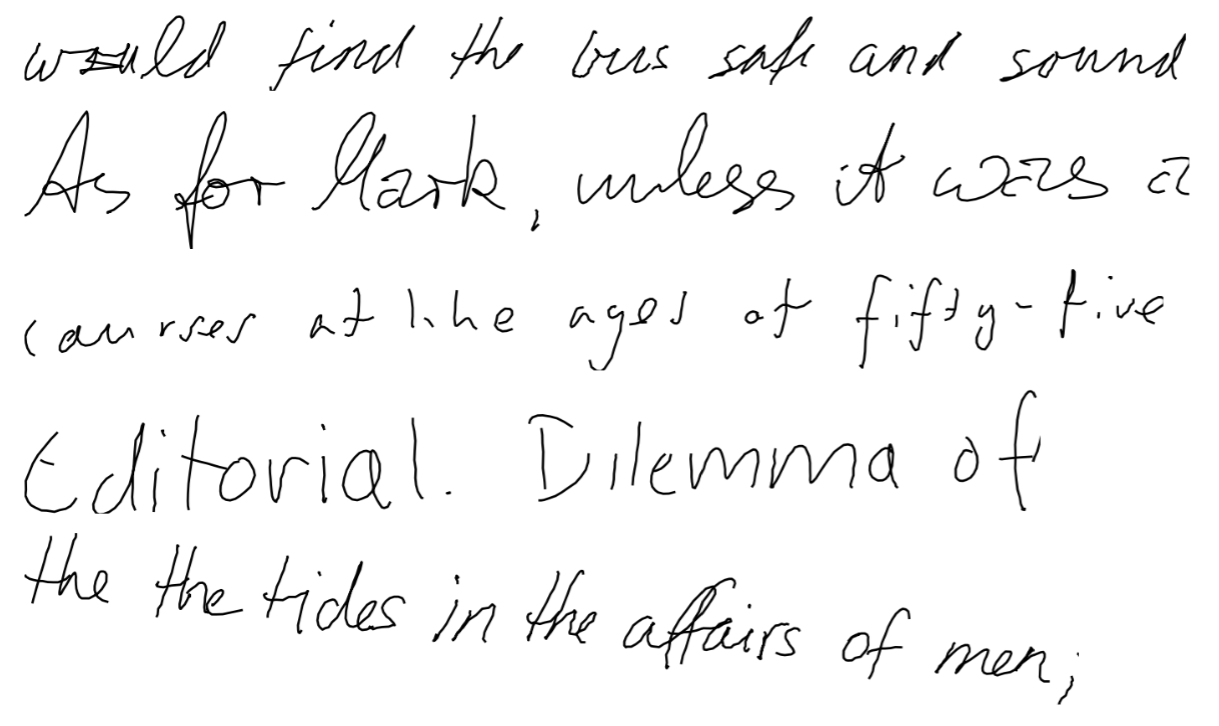
\includegraphics[width=7cm]{./imag/iam.png}
\end{center}
\pause
\\[5pt]
\textbf{Generated data:}
\begin{center}
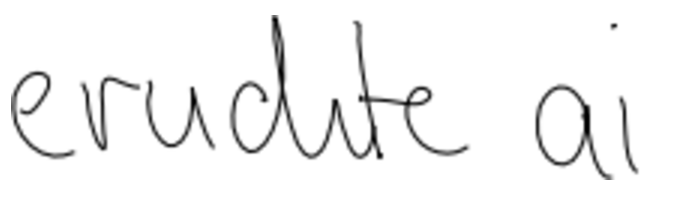
\includegraphics[width=5cm]{./imag/erudite_handwriting.png}
\end{center}
\end{frame}

\begin{frame}{Deep recurrent neural network architecture}

\begin{center}
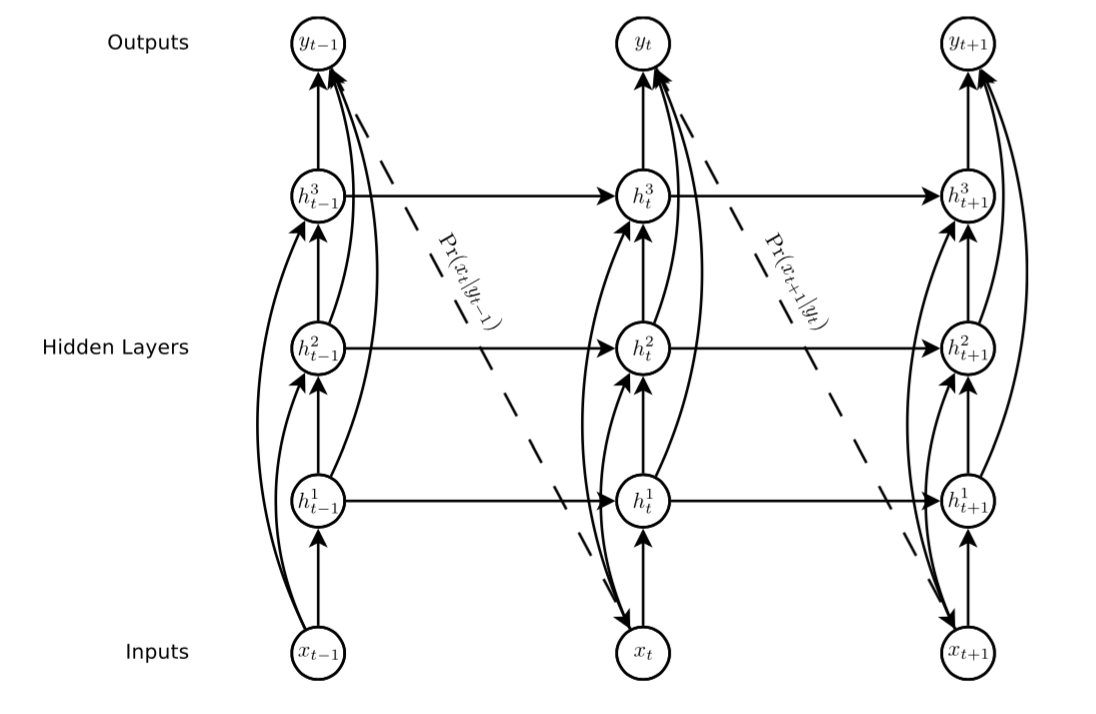
\includegraphics[width=10cm]{./imag/architecture.png}
\end{center}

\footnotetext{Image taken from the article Generating Sequences with recurrent neural networks from Alex Graves https://arxiv.org/abs/1308.0850}
%\pause

\end{frame}

\begin{frame}{Long-Short Term Memory architecture uses purpose-built memory cells to learn long term dependencies}
\begin{center}
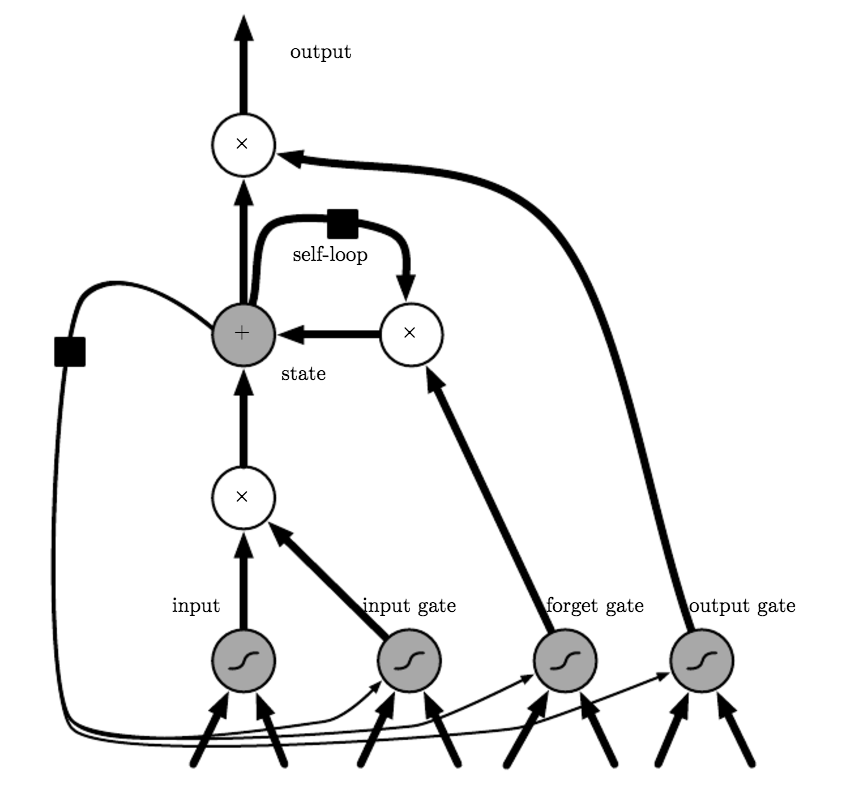
\includegraphics[width=7cm]{./imag/lstm.png}
\end{center}
\footnotetext{Image taken from the book Deep Learning by Goodfellow et al. http://www.deeplearningbook.org/}
\end{frame}

\begin{frame}{The text model takes the softmax function of the last layer and calculates the loss function using cross-entropy}
\begin{center}
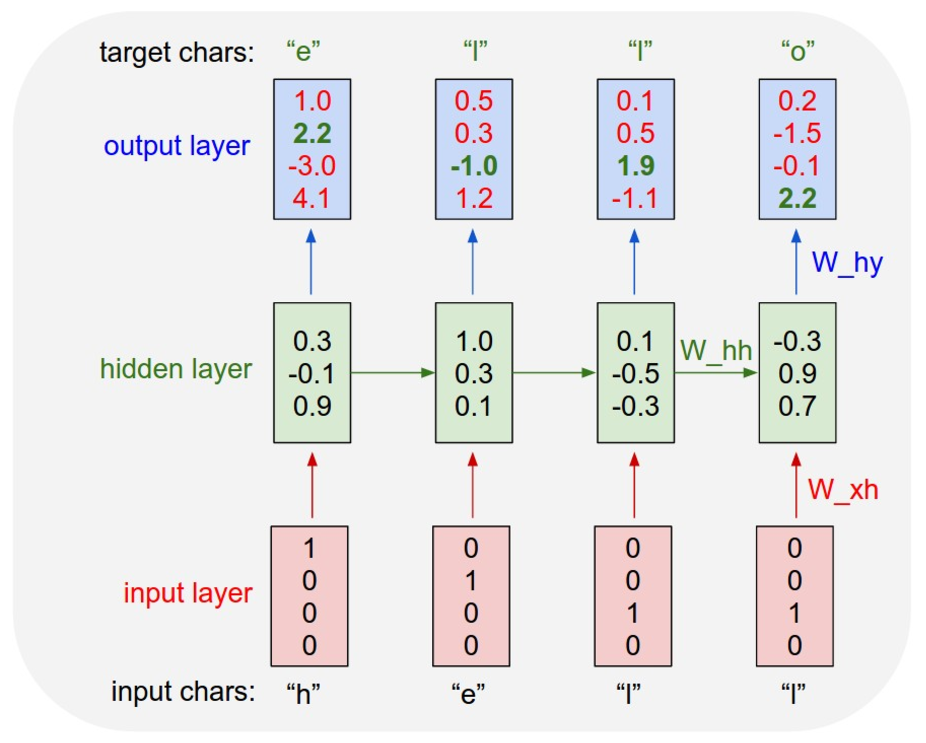
\includegraphics[width=8cm]{./imag/rnn.png}
\end{center}
\footnotetext{Image taken from Andrej Karapathy's blog http://karpathy.github.io/2015/05/21/rnn-effectiveness/}
\end{frame}

\begin{frame}{Examples of character-level text generation}

\fbox{\begin{minipage}{30em}
And the mighty of it is a standed me with the things the first the wicked in the sons of Saul the play of the word of the son of Kanah, and at the singer of the morning that have in the word of the LORD and the word of the LORD and the standing of the LORD, and went in the people came out of God.
\end{minipage}}
\\[10pt]
\pause
\fbox{\begin{minipage}{30em}
KING LEAR:
O, if you were a feeble sight, the courtesy of your law,
Your sight and several breath, will wear the gods
With his heads, and my hands are wonder'd at the deeds,
So drop upon your lordship's head, and your opinion
Shall be against your honour.
\end{minipage}}
\footnotetext{Shakespeare's generation taken from Andrej Karapathy's blog http://karpathy.github.io/2015/05/21/rnn-effectiveness/}
\end{frame}



\begin{frame}{Online handwriting: IAM database}
\begin{center}
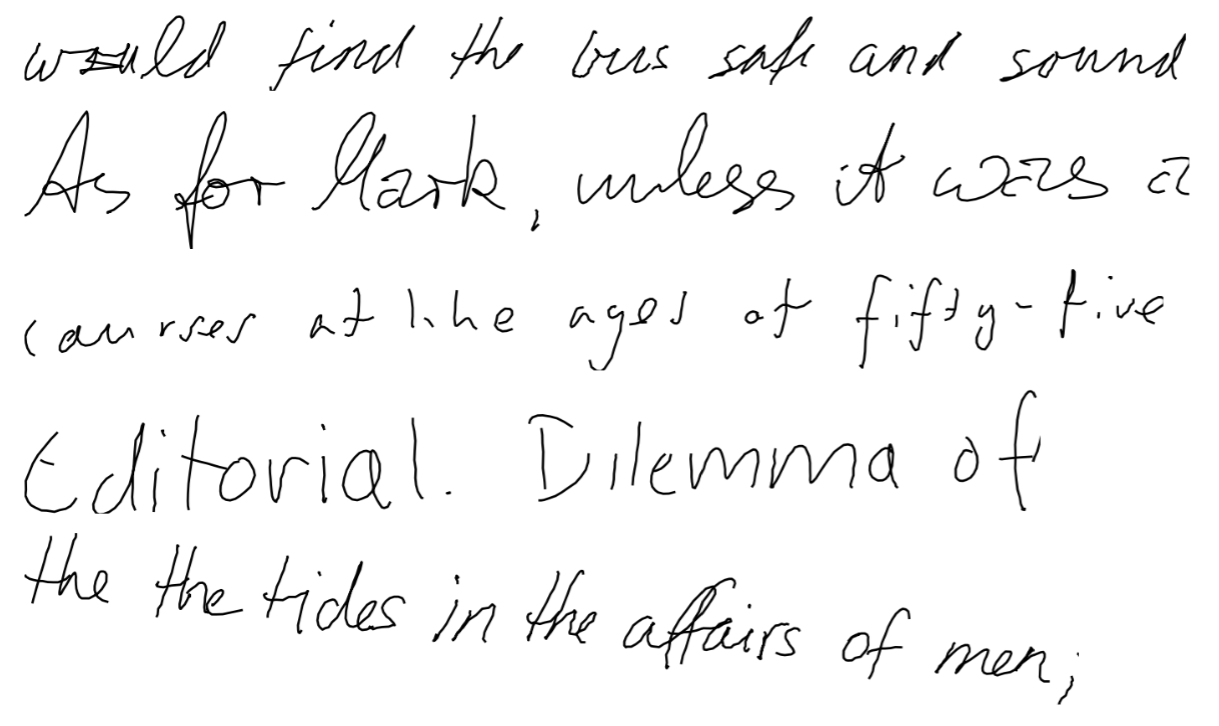
\includegraphics[width=10cm]{./imag/iam.png}
\end{center}
\footnotetext{Image taken from the article Generating Sequences with recurrent neural networks from Alex Graves https://arxiv.org/abs/1308.0850}
\end{frame}

\begin{frame}{Online handwriting: database format}
\begin{center}
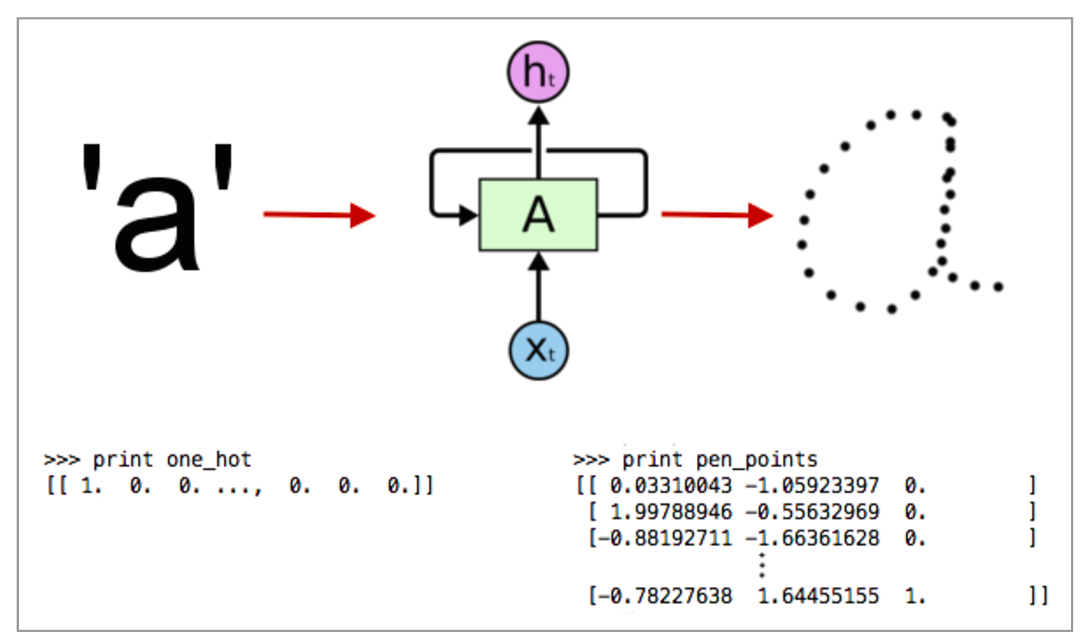
\includegraphics[width=10cm]{./imag/handwriting.png}
\end{center}
\footnotetext{Image taken from Sam Greydanus' blog https://greydanus.github.io/2016/08/21/handwriting/}
\end{frame}

\begin{frame}{Model for online handwriting}
\begin{center}
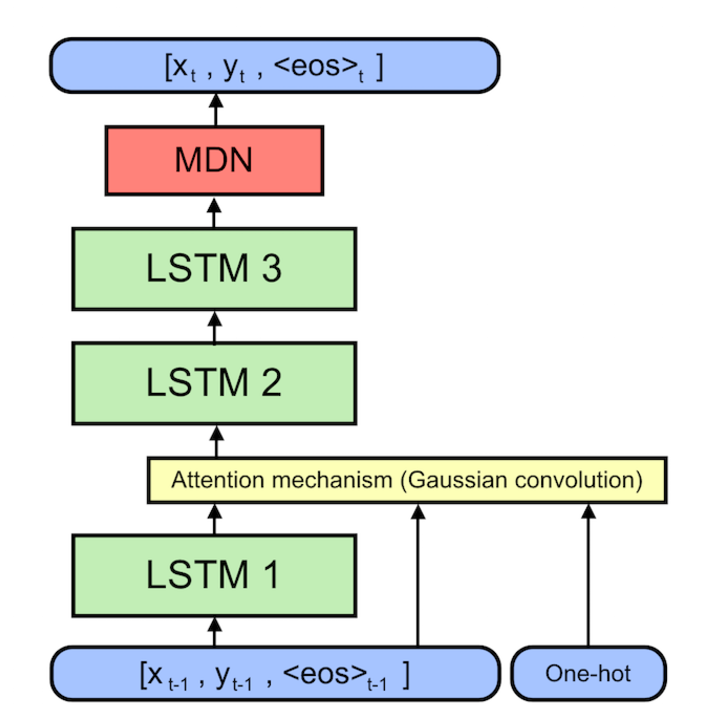
\includegraphics[width=6cm]{./imag/mdn.png}
\end{center}
\footnotetext{Image taken from Sam Greydanus' blog https://greydanus.github.io/2016/08/21/handwriting/}
\end{frame}

\begin{frame}{Results of Online Handwriting}
\begin{center}
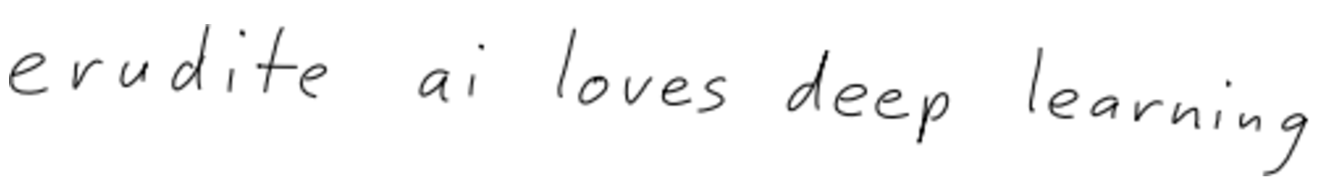
\includegraphics[width=11cm]{./imag/dl.png}
\end{center}
\pause
\begin{center}

\includegraphics[width=11cm]{./imag/montreal.png}
\end{center}
\pause
\begin{center}

\includegraphics[width=11cm]{./imag/listening.png}
\end{center}
\footnotetext{Handwriting created using Alex Graves' generation demo http://www.cs.toronto.edu/~graves/handwriting.html}
\end{frame}

\begin{frame}{Discussion time}
    Questions, thoughts or comments?
\end{frame}

\end{document}
